\chapter{Introduction}\label{sec:intro}

\section{Context and state of the art}

\paragraph{Modeling.}
As the title suggests this work deals with modeling and control of rigid body systems.
The procedure of physical modeling is illustrated in \autoref{fig:ModelingIllustration}.
It starts by approximating the system under consideration by a mechanical model.
The mathematical part requires the choice of coordinates $\sysState$ to capture the state (positions and velocities) of the model.
Combining this with principles of mechanics, we may derive a set of ordinary differential equations that capture its motion.
This work mainly deals with this second part, i.e.\ the derivation of \textit{equations of motion}.
%Since there is generally an infinite set of possible parameterizations for a rigid body model, the equations of motion are not unique.

\begin{figure}[ht]
 \centering
 %\footnotesize
 \newcommand{\ModelingIllustrationOde}{$\dot{\sysState}=\tuple{f}(\sysState,\sysInput)$}
 \appendtographicspath{{graphics/ModelingIllustration/}}
 \input{graphics/ModelingIllustration/ModelingIllustration.pdf_tex}
 \caption{Modeling illustration}
 \label{fig:ModelingIllustration}
\end{figure}

A very common approach for deriving equations of motion of finite-demensional, holonomic mechanical systems is the so called \textit{Lagrange formalism}:
First, the system is parameterized by so called \textit{generalized coordinates} $\genCoord$.
Then the kinetic energy $\kineticEnergy$, the potential energy $\potentialEnergy$ and virtual work $\delta \mathcal{W}$ of external forces are formulated in terms of these coordinates and their derivatives $\genCoordd = \sfrac{\d \genCoord}{\d t}$:
\begin{align}
 \Lagrangian(\genCoord, \genCoordd) = \kineticEnergy(\genCoord, \genCoordd) - \potentialEnergy(\genCoord),
\qquad
 \delta\mathcal{W}^{\text{E}} = (\delta\genCoord)^\top \genForceEx.
\end{align}
The equations of motion are derived from the Lagrangian $\Lagrangian$ as
\begin{align}\label{eq:LagrangeEq}
 \diff{t} \pdiff[\Lagrangian]{\genCoordd} - \pdiff[\Lagrangian]{\genCoord} = \genForceEx.
\end{align}
The kinetic energy for a time-invariant, mechanical system is always strictly quadratic $\kineticEnergy = \tfrac{1}{2} \genCoordd^\top \sysInertiaMat(\genCoord)\genCoordd$.
Furthermore, we assume that the external forces $\genForceEx$ is an affine function of the control inputs $\sysInput$.
Then the equations of motion take the structure
\begin{align}\label{eq:introEqOfMotion}
 \sysInertiaMat(\genCoord)\genCoorddd + \sysForce(\genCoord,\genCoordd) = \sysInputMat(\genCoord) \sysInput
\qquad \Leftrightarrow \qquad
 \tdiff{t} \underbrace{\begin{bmatrix} \genCoord \\ \genCoordd \end{bmatrix}}_{\sysState}
 = \underbrace{\begin{bmatrix} \genCoordd \\ \sysInertiaMat^{-1}(\genCoord)(\sysInputMat(\genCoord) \sysInput - \sysForce(\genCoord,\genCoordd)) \end{bmatrix}}_{\tuple{f}(\sysState,\sysInput)}
\end{align}
The right hand side of \eqref{eq:introEqOfMotion} is a standard form for simulation, i.e.\ numerical solution, or general control design.
However, the structure of the left hand side of \eqref{eq:introEqOfMotion} can be exploited for a particular control design.

\paragraph{Feedback Control.}
From a mathematical point of view, a feedback controller is some map $\sysInput = \tuple{g}(\sysState,\tuple{r})$ that computes the control input $\sysInput$ based on the measured system state $\sysState$ and some reference input $\tuple{r}$.
The goal is that the resulting controlled system $\dot{\sysState} = \tuple{f}(\sysState,\tuple{g}(\sysState,\tuple{r})) = \bar{\tuple{f}}(\sysState,\tuple{r})$ has desirable properties.

\begin{figure}[ht]
 \centering
 \newcommand{\macCtrlBlockKinetics}{$\dot{\sysState} = \tuple{f}(\sysState,\sysInput)$}
 \newcommand{\macCtrlBlockCtrl}{$\sysInput = \tuple{g}(\sysState, \tuple{r})$}
 \newcommand{\macControlBlockClosedLoopKinetics}{$\dot{\sysState} = \bar{\tuple{f}}(\sysState,\tuple{r})$}
 \newcommand{\macCtrlBlockMeas}{$\sysState$}
 \newcommand{\macCtrlBlockInput}{$\sysInput$}
 \newcommand{\macCtrlBlockRef}{$\tuple{r}$}
 \newcommand{\macCtrlBlockInitials}{$\sysState(t_0)$}
 \input{graphics/introCtrlBlock.pdf_tex}
 \caption{Model, controller and controlled system}
 \label{fig:introCtrlBlock}
\end{figure}

For a system of the structure \eqref{eq:introEqOfMotion}, a typical control objective is, that a given reference trajectory $t \mapsto \genCoordR(t)$ is a stable trajectory of the controlled system.
If there are as many control inputs as degrees of freedom $\dim\sysInput = \dim\genCoord = \dimConfigSpace$ and the input matrix $\sysInputMat$ is invertible, there is a popular control approach, commonly called \textit{computed torque}:
Defining the error dynamics as
\begin{align}
 \ddot{\tuple{e}} + \mat{\Lambda}_1 \dot{\tuple{e}} + \mat{\Lambda}_0 \tuple{e} = \tuple{0}, \quad \tuple{e} = \genCoord - \genCoordR
\end{align}
with the symmetric, positive definite matrices $\mat{\Lambda}_0, \mat{\Lambda}_1$ as tuning parameters.
Combining this with the model \eqref{eq:introEqOfMotion} yields the control law
\begin{align}
 \sysInput = \sysInputMat^{-1} \big( \sysInertiaMat(\genCoord)(\genCoordRdd - \mat{\Lambda}_1 \dot{\tuple{e}} - \mat{\Lambda}_0 \tuple{e}) + \sysForce(\genCoord,\genCoordd) \big)
 = \tuple{g}\big( \underbrace{\genCoord, \genCoordd}_{\sysState}, \underbrace{\genCoordR, \genCoordRd, \genCoordRdd}_{\tuple{r}} \big)
\end{align}

\paragraph{Multicopters.}
In contrast to conventional helicopters, multicopters are aerial vehicles that use several rigid (fixed pitch) propellers to generate lift and maneuver.
They are usually small and unmanned and are used to carry cameras or other sensors.
In particular, the four propeller quadcopter configuration has became quite popular over the last two decades.

\begin{figure}[ht]
 \centering
 \input{graphics/lsrMulticopters.pdf_tex}
 \caption{lsr-quadcopter (left), lsr-tricopter (middle) and a concept of a bicopter}
 \label{fig:introLsrMulticopters}
\end{figure}

The \textit{Chair of Systems Theory and Control Engineering} at Saarland University has developed realizations of a quadcopter and a tricopter with three tiltable propellers (see \autoref{fig:introLsrMulticopters}).
A bicopter with two titlable and inclined propellers has been studied through simulations.
In particular the lsr-quadcopter has an excellent thrust to weight ratio and is consequently well suited for aggressive, aerobatic maneuvers, e.g. a looping as shown in \autoref{fig:introQuadLoopSnapshots}.

\begin{figure}[ht]
 \centering
 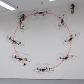
\includegraphics{graphics/QuadLoopSnapshots}
 \caption{Snapshots of the lsr-quadcopter tracking a looping trajectory}
 \label{fig:introQuadLoopSnapshots}
\end{figure}

From a mechanical point of view, these multicopters may be modelled as a free rigid body moving within Earth's gravity.
The difference between them is only the placement of the actuators:
the tricopter is fully-actuated, so it poses the easiest control task.
The quadcopter only has four actuators for its six degrees of freedom, i.e. it is underactuated.
However, its model is well known to be a configuration flat system and corresponding standard control design approaches may be applied.
The bicopter is (probably) not a flat system and consequently, poses the toughest control task.


\section{Motivation example}\label{sec:MotivationRigidBodyAttitude}
Consider a free rigid body as illustrated in the middle of \autoref{fig:ModelingIllustration}, but fixed at its center of mass, i.e.\ it may only rotate about this point.
For simplicity, we also assume that the chosen frame coincides with its principle axis and there are three independent control torques about these axis.
Then the coefficients of inertia are $\J = \diag(\Jx,\Jy,\Jz)$.

\paragraph{Lagrange's equation.}
For application of the Lagrange formalism we need to parameterize the system by minimal generalized coordinates.
A popular choice for the rigid body orientation are Euler angles in the \textit{roll-pitch-yaw} convention:
\begin{subequations}\label{eq:EulerAngleParam}
\begin{align}
 \R(\genCoord) &=
 \begin{bmatrix}
  \cyaw \cpit & -\syaw \crol+\cyaw \spit \srol & \syaw \srol+\cyaw \spit \crol \\
  \syaw \cpit & \cyaw \crol+\syaw \spit \srol & -\cyaw \srol+\syaw \spit \crol \\
  -\spit & \cpit \srol & \cpit \crol  
 \end{bmatrix},
 \label{eq:EulerAngleParamR}
\\
 \w(\genCoord, \genCoordd) &=
 \underbrace{\begin{bmatrix}
  1 & 0 & -\spit \\
  0 & \crol & \cpit \srol \\
  0 & -\srol & \cpit \crol
 \end{bmatrix}}_{\kinBasisMat(\genCoord)}
 \underbrace{\begin{bmatrix} \rold \\ \pitd \\ \yawd \end{bmatrix}}_{\genCoordd}.
 \label{eq:EulerAngleParamW}
\end{align}
\end{subequations}
The shortcut notation $\syaw := \sin(\yaw)$ and $\cyaw := \cos(\yaw)$ used here, will be used throughout this text.
With this, we may formulate the kinetic energy $\kineticEnergy(\genCoord, \genCoordd) = \tfrac{1}{2} (\w(\genCoord, \genCoordd))^\top \J \w(\genCoord, \genCoordd)$ which coincides with the Lagrangian since there is no potential energy.
% \begin{align}
%  \kineticEnergy(\genCoord, \genCoordd)
%  = \tfrac{1}{2} (\w(\genCoord, \genCoordd))^\top \J \, \w(\genCoord, \genCoordd)
%  = \tfrac{1}{2} \genCoordd^\top \underbrace{(\kinBasisMat(\genCoord))^\top \J \, \kinBasisMat(\genCoord)}_{\sysInertiaMat(\genCoord)} \genCoordd,
% \end{align}
Evaluation of Lagrange's equation \eqref{eq:LagrangeEq} yields the equations of motion 
\begin{multline}\label{eq:LagrangeEqRBAttitude}
 \underbrace{\begin{bmatrix}
  \Jx & 0 & -\Jx \spit \\
  0 & \Jy\crol^2 + \Jz\srol^2 & (\Jy-\Jz)\crol\srol\cpit \\
  -\Jx \spit & (\Jy-\Jz)\crol\srol\cpit & \Jx\spit^2 + (\Jy\srol^2 + \Jz\crol^2)\cpit^2 
 \end{bmatrix}}_{\sysInertiaMat(\genCoord)}
 \underbrace{\begin{bmatrix} \roldd \\ \pitdd \\ \yawdd \end{bmatrix}}_{\genCoorddd}
\\
 + \underbrace{\begin{bmatrix}
  (\Jy-\Jz)\crol\srol \pitd^2 + \cdots \\ %(2(\Jz-\Jy)\crol^2 - \Jx + \Jy - \Jz)\cpit \yawd \pitd + \ldots \\%(-(\cpit)^2 \srol \Jy \crol+(\cpit)^2 \crol \Jz \srol) \yawd^2 \\
  2(\Jz-\Jy)\srol\crol\pitd \rold + \cdots \\ %((2 (\Jy-\Jz)\crol^2 + \Jx - \Jy + \Jz)\cpit \yawd)\rold + \ldots \\%(-\Jy \cpit (\crol)^2 \spit+\cpit (\crol)^2 \Jz \spit-\spit \Jx \cpit+\Jy \cpit \spit) \yawd^2 \\
  (2(\Jy-\Jz)\crol^2 - \Jx - \Jy + \Jz)\cpit \pitd \rold + \cdots \\ % (2(\Jy-\Jz) \cpit^2 \crol \srol \yawd) \rold + \ldots %(-\crol \Jy \spit \srol+\srol \Jz \spit \crol) \pitd^2+(2 \Jy \cpit (\crol)^2 \spit-2 \cpit (\crol)^2 \Jz \spit+2 \spit \Jx \cpit-2 \Jy \cpit \spit) \yawd \pitd
 \end{bmatrix}}_{\sysForce(\genCoord, \genCoordd)}
% = \underbrace{\begin{bmatrix} 0 & \ArmRadius & 0 & -\ArmRadius \\ \PropTorqueFaktor\srol - \ArmRadius\crol & -\PropTorqueFaktor\srol & \PropTorqueFaktor\srol + \ArmRadius\crol & -\PropTorqueFaktor\srol \\ -\PropTorqueFaktor\crol\cpit - \ArmRadius\srol\cpit & \PropTorqueFaktor\crol\cpit - \ArmRadius\cpit & -\PropTorqueFaktor\crol\cpit - \ArmRadius\srol\cpit & \PropTorqueFaktor\crol\cpit + \ArmRadius\cpit \end{bmatrix}}_{\sysInputMat(\genCoord)}
% \underbrace{\begin{bmatrix} u_1 \\ u_2 \\ u_3 \\ u_4 \end{bmatrix}}_{\sysInput}.
 = \underbrace{\begin{bmatrix}
  1 & 0 & 0 \\
  0 & \crol & -\srol \\
  -\spit & \cpit \srol & \cpit \crol
 \end{bmatrix}}_{\kinBasisMat^\top(\genCoord)}
 \underbrace{\begin{bmatrix} \taux \\ \tauy \\ \tauz \end{bmatrix}}_{\sysInput}.
\end{multline}
The entries in $\sysForce$ are not displayed here since they would fill several lines and are actually not of relevance here.
What is crucial here is that the model has singularities at $\pit=\pm\tfrac{\pi}{2}$: $\det\sysInertiaMat = \Jx\Jy\Jz\cpit^2$ and $\det\kinBasisMat = \cpit$.
For the previous example of aerobatic motions it is should be evident that singularities of this form would be unacceptable for simulation and control design. 

%Consequently this model is neither suited for a global simulation nor for application of computed torque control.

\paragraph{Euler's rotation equations.}
For the particular example of the rigid body orientation one finds another formulation of the equations of motion directly in most textbooks on mechanics, e.g.\ \cite[p.\,143]{Arnold:MathematicalMethodsOfClassicalMechanics} or \cite[p.\,145]{Schwertassek:MultibodySystems}:
%They are commonly called \textit{Euler's rotation equations}:
\begin{subequations}\label{eq:ExampleEulerEq}
\begin{align}
 \ddt
 \underbrace{\begin{bmatrix} \Rxx & \Rxy & \Rxz \\ \Ryx & \Ryy & \Ryz \\ \Rzx & \Rzy & \Rzz \end{bmatrix}}_{\R}
 =
 \underbrace{\begin{bmatrix} \Rxx & \Rxy & \Rxz \\ \Ryx & \Ryy & \Ryz \\ \Rzx & \Rzy & \Rzz \end{bmatrix}}_{\R}
 \underbrace{\begin{bmatrix} 0 & -\wz & \wy \\ \wz & 0 & -\wx \\ -\wy & \wx & 0\end{bmatrix}}_{\wedOp{\w}},
\label{eq:ExampleEulerEqKinematics}
\\
 \underbrace{\begin{bmatrix} \Jx & 0 & 0 \\ 0 & \Jy & 0 \\ 0 & 0 & \Jz \end{bmatrix}}_{\J}
 \underbrace{\begin{bmatrix} \wxd \\ \wyd \\ \wzd \end{bmatrix}}_{\dot{\w}}
 + \underbrace{\begin{bmatrix} 0 & -\wz & \wy \\ \wz & 0 & -\wx \\ -\wy & \wx & 0\end{bmatrix}}_{\wedOp{\w}}
 \underbrace{\begin{bmatrix} \Jx & 0 & 0 \\ 0 & \Jy & 0 \\ 0 & 0 & \Jz \end{bmatrix}}_{\J}
 \underbrace{\begin{bmatrix} \wx \\ \wy \\ \wz \end{bmatrix}}_{\w}
 = 
 \underbrace{\begin{bmatrix} \taux \\ \tauy \\ \tauz \end{bmatrix}}_{\sysInput}.
 %\underbrace{\begin{bmatrix} 0 & \ArmRadius & 0 & -\ArmRadius \\ -\ArmRadius & 0 & \ArmRadius & 0 \\ -\PropTorqueFaktor & \PropTorqueFaktor & -\PropTorqueFaktor & \PropTorqueFaktor \end{bmatrix}}_{\sysInputMat}
 %\underbrace{\begin{bmatrix} u_1 \\ u_2 \\ u_3 \\ u_4 \end{bmatrix}}_{\sysInput}.
 \label{eq:ExampleEulerEqKinetics}
\end{align}
\end{subequations}
The 9 coefficients of the matrix $\R$ have to obey the constraint $\R^\top \R = \idMat[3]$.
However, it can be shown that if this is fulfilled for the initial condition $\R(t_0)$, then the kinematic equation \eqref{eq:ExampleEulerEqKinematics} ensures that the condition remains fulfilled.
This formulation has no singularities and is well suited for global simulation.
Moreover, loosely speaking, its mathematical structure reflects the physical symmetries of the model.
The obvious draw-back is that due to the lack of generalized coordinates, its unclear how a method like computed torque could be applied.

\paragraph{Discussion.}
Euler's equations \eqref{eq:ExampleEulerEq} and \eqref{eq:LagrangeEqRBAttitude} describe the same system.
In fact one may plug \eqref{eq:EulerAngleParamW} into \eqref{eq:ExampleEulerEqKinetics} and multiply it by $\kinBasisMat^\top$ to obtain \eqref{eq:LagrangeEqRBAttitude}.

Each of these formulations has its advantages and draw-backs:
Euler's equations are more compact and have a symmetric structure in contrast to \eqref{eq:LagrangeEqRBAttitude}.
The downside is that they require 9 coordinates, the coefficients of the rotation matrix $\R$, to parameterize the attitude, whereas the Euler-angles $\genCoord$ only require 3.
The crucial advantage of Lagrange's equation \eqref{eq:LagrangeEq} is, that it holds for \textit{any} finite dimensional and holonomic mechanical system, whereas Euler's equations only hold for this particular example.
However, for this example, the equations \eqref{eq:LagrangeEqRBAttitude} are quite cumbersome and lack an obvious structure.
Probably the worst fact is that the inertia matrix $\sysInertiaMat(\genCoord)$ is singular at the point $\pit=\pm\tfrac{\pi}{2}$ and consequently $\genCoorddd$ is undefined at these points.

It should be stressed that there is no physical reason for the singularity in the Lagrangian version \eqref{eq:LagrangeEqRBAttitude}, it is rather a consequence of an unsuitable parameterization of the system.
This is pointed out in \cite[sec.\ 1.1.1]{Schwertassek:MultibodySystems} as:
\textit{
[The scientists of the Eighteenth Century] recognized that there was something about rotation [\ldots] which somehow made the analysis of rotation a problem of higher order difficulty. 
We now know that the problem is in the mathematics, not the physics, but the problem is still with us.
}

The set of 3-dimensional rotation matrices $\R\in\SpecialOrthogonalGroup(3)$ captures the actual configuration space of the rigid body orientation well, but it is difficult to work with since the coefficients of the rotation matrix are not independent.
Since $\R\in\SpecialOrthogonalGroup(3)$ is compact while $\RealNum^3$ is not, there is no bijection between them, see also \cite[sec.\ 1.1d]{Frankel:GeometryOfPhysics}.
The chosen set of Euler angles may be regarded as a surjective but not injective function from $\RealNum^3$ to $\R\in\SpecialOrthogonalGroup(3)$ in a similar manner as latitude and longitude serve as coordinates for Earth's surface. 
The Euler angles are unsuited at the so called gimbal lock ($\pit=\pm 90^\circ$) just as longitude fails at Earths poles.


\section{Goal and outline of this work}
The first chapter reviews established methods of analytical mechanics with the addition of allowing redundant coordinates (like the coefficients of a rotation matrix $\R$) and nonholonomic velocity coordinates (like the coefficients of the angular velocity $\w$).
It will present a formulation that can derive both of the presented equations of motion for the motivation example, but holds for general finite-dimensional mechanical systems.

The second chapter specializes to rigid body systems, i.e. systems that consist of several interconnected rigid bodies.
It presents an algorithm that derives the equations of motion based on chosen coordinates and given constitutive parameters.
Furthermore, natural formulations of stiffness, dissipation and inertia for a rigid body are established.

The third chapter proposes tracking control algorithms for rigid body systems.
Based on the findings of the second chapter it will present three control algorithms motivated by defining desired stiffness, damping and inertia of the resulting controlled system.
Furthermore, these algorithms are extended to tackle underactuated systems.
These algorithms are discussed through several examples.

The fourth chapter presents the developed quadcopter and tricopter and their performance for real control of aerobatic maneuvers.

